\chapter{Simulações e resultados}
	Neste capítulo, serão apresentados os resultados experimentais de todo o processo de obtenção do efeito de \textit{Reverb Shimmer}, bem como alguns resultados de testes de pequenos algortimos implementados no microcontrolador MSP430F5529 com seu conversor Analógico Digital de 12 bits e a comunicação I$ ^2 $C entre o $ \mu C $ e o dispositivo MCP 4725.
	
	\section{Descrição dos Experimentos}
	
		Os experimentos ora mostrados foram realizados de forma a demonstrar toda a abordagem de aprendizagem durante o projeto. Conforme será explicado na conclusão do trabalho, posto que foi identificado, através de experimento e cálculos realizados na implementação as limitações do hardware proposto para a execução do código do efeito digital em si.


		Os resultados das simulações serão divididos da seguinte ordem:
		
		\begin{enumerate}
			\item Comparativo da quantização de um sinal de aúdio com resoluções de 16 e 12 bits;
			\item Comparativo da quantização de um sinal de aúdio com resoluções de 12, 10 e 8 bits;
			\item 
		\end{enumerate}
	
		Para os experimentos acima mencionados serão utilizados os seguintes dados mostrado na tabela \ref{tab-exp01}:
		
		\begin{table}[!ht]
			\centering
			\begin{tabular}[ht!]{|c|c|}
				\hline 
				Fonte de Áudio		&	\textit{'guitar-clean16.wav'} - som de guitarra limpa\\
				\hline
				Taxa de Amostragem 	&	44100 Hz	\\
				\hline
				Número de Canais 	&	1 canal mono\\ 
				\hline
			\end{tabular}
			\caption{Dados relativos as simulações no computador}
			\label{tab-exp01}
		\end{table}
		
		
		Esses resultados das figuras  são apenas a título de informações preliminares na escolha da resolução adequada para que o sinal seja tratado posteriormente no microcontrolador. Nesse caso, posto que o conversor em questão seja de 12 (doze) \textit{bits} percebe-se que não há uma perda significativa na resolução do sinal, bem como audivelmente não se percebeu grande perda de qualidade em relação ao áudio original em 16 \textit{bits}.
		
		\begin{figure}[!ht]
			\label{fig-exp2}
			\centering
			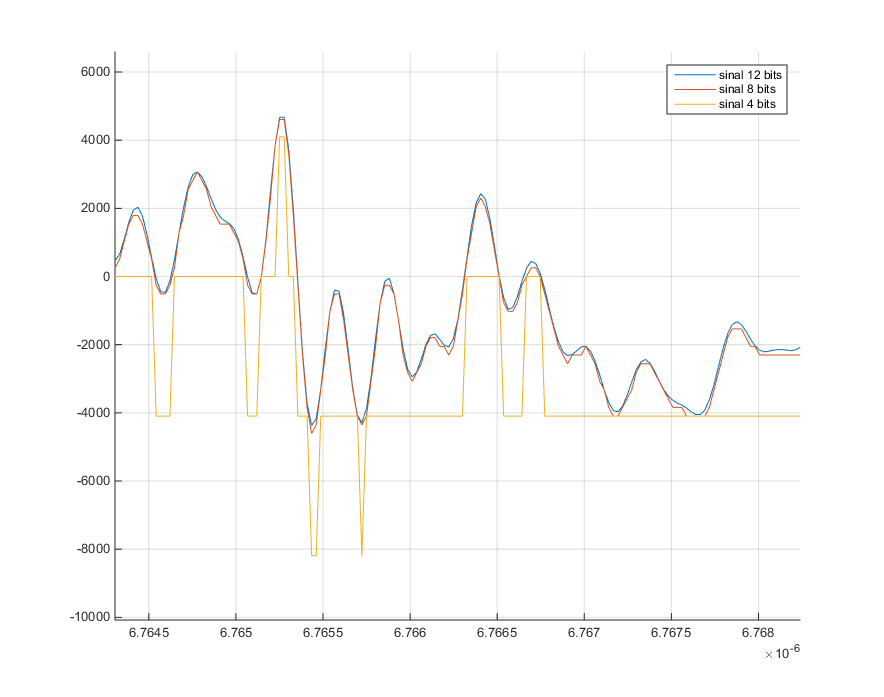
\includegraphics[scale=0.5]{./figuras/simulacoes/resolucao-audios/12-8-4-normal.png}
			\caption{Quantização do sinal de áudio em 12, 8 e 4 bits PCM}
		\end{figure}
		
		\begin{figure}[!ht]
			\label{fig-exp1}
			\centering
			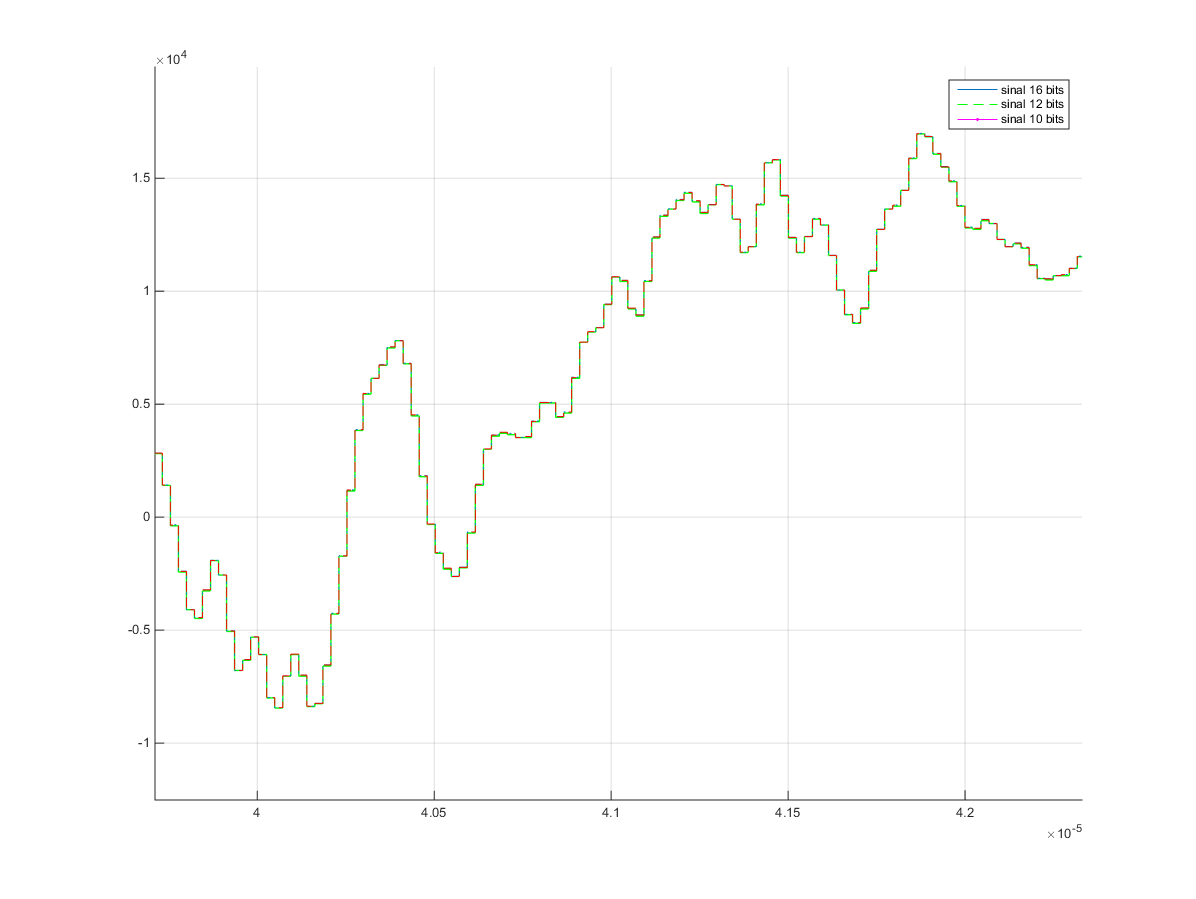
\includegraphics[scale=0.5]{./figuras/simulacoes/resolucao-audios/10-12-16-normal.png}
			\caption{Quantização do sinal de áudio em 10, 12 e 16 bits PCM}
		\end{figure}
	
		\begin{figure}[!ht]
			\label{fig-exp3}
			\centering
			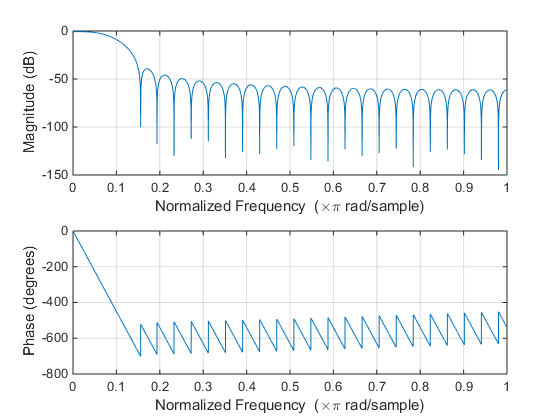
\includegraphics[scale=0.7]{./figuras/simulacoes/resposta-do-filtro-FIR-FPB-2khz.png}
			\caption{Resposta do filtro FIR-Passa-Baixa com janela \textit{Blackman}}
		\end{figure}
	
		Essa resposta do filtro passa baixa (figura \ref{fig-exp3}) com frequência de corte igual a 2kHz. Esse filtro foi utilizado o número de 51 \textit{Taps}. Nota-se que a atenuação começa a partir da frequência $f_{[\rm rad/samples]} = f_{[\rm cycles/sec]}\cdot \frac{\text{sec}}{\text{samples}}\cdot \frac{\text{rad}}{\text{cycle}} \Rightarrow f_{[\rm rad/samples]} = f_{[\rm cycles/sec]}\cdot \frac{2\pi}{f_s}\Rightarrow f = 44100*0.2/2\pi = 1403.74 Hz$.
	
		
		A seguir temos nas figuras \ref{fig:impulse-reverb} e \ref{fig:warhouse-impulse-reverb} os áudios para serem utilizados no processo de convolução com o sinal original, originando o efeito de reverb em convolução.
		
		\begin{figure}[th]
			\centering
			\subfigure[Espectro de frequência de uma resposta impulsional de um som oriundo do Palácio de \textit{Falkland Palace in Fife}.]{
			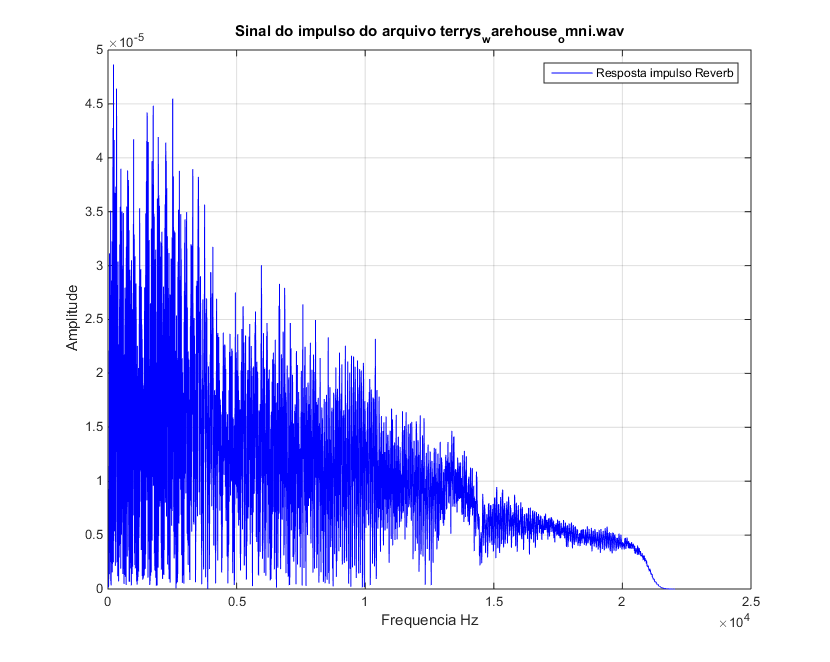
\includegraphics[width=0.7\linewidth]{figuras/simulacoes/impulse-reverb}
			\label{fig:impulse-reverb}
			}
			
			\subfigure[Espectro de frequência de uma resposta impulsional de um som oriundo de uma \textit{empty warehouse} (armazem vazio).]{
			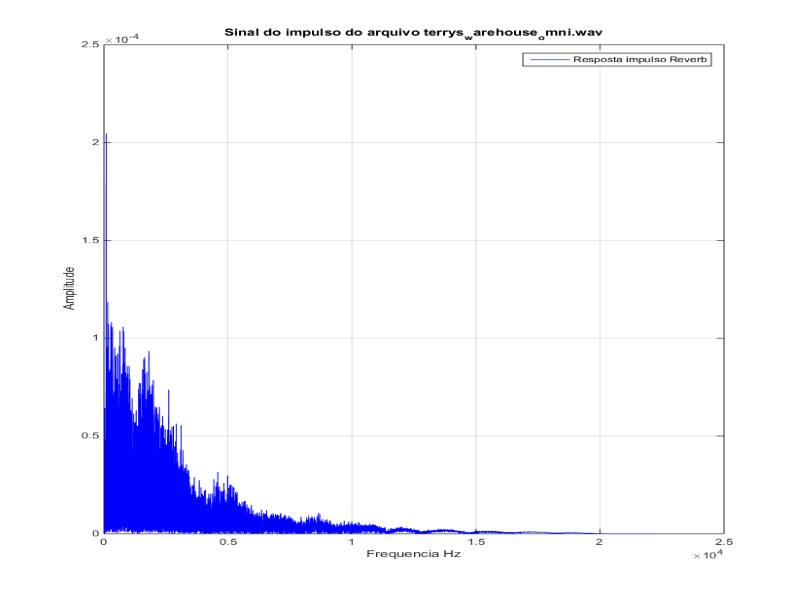
\includegraphics[width=0.7\linewidth]{figuras/simulacoes/warhouse-impulse-reverb}
			\label{fig:warhouse-impulse-reverb}
			}	
			\caption{Respostas Impulsionais de Ambiente: Exemplos retirado do \textit{website}: \href{http://www.openairlib.net/}{OpenAir}.}
		\end{figure}
	
		Resultado da resposta em frequência (figura \ref{fig-sinal12bits-filtrado}) da aplicação do filtro FIR-passa-baixa no sinal original de 12 bits:
		
		\begin{figure}[!ht]
			\centering
			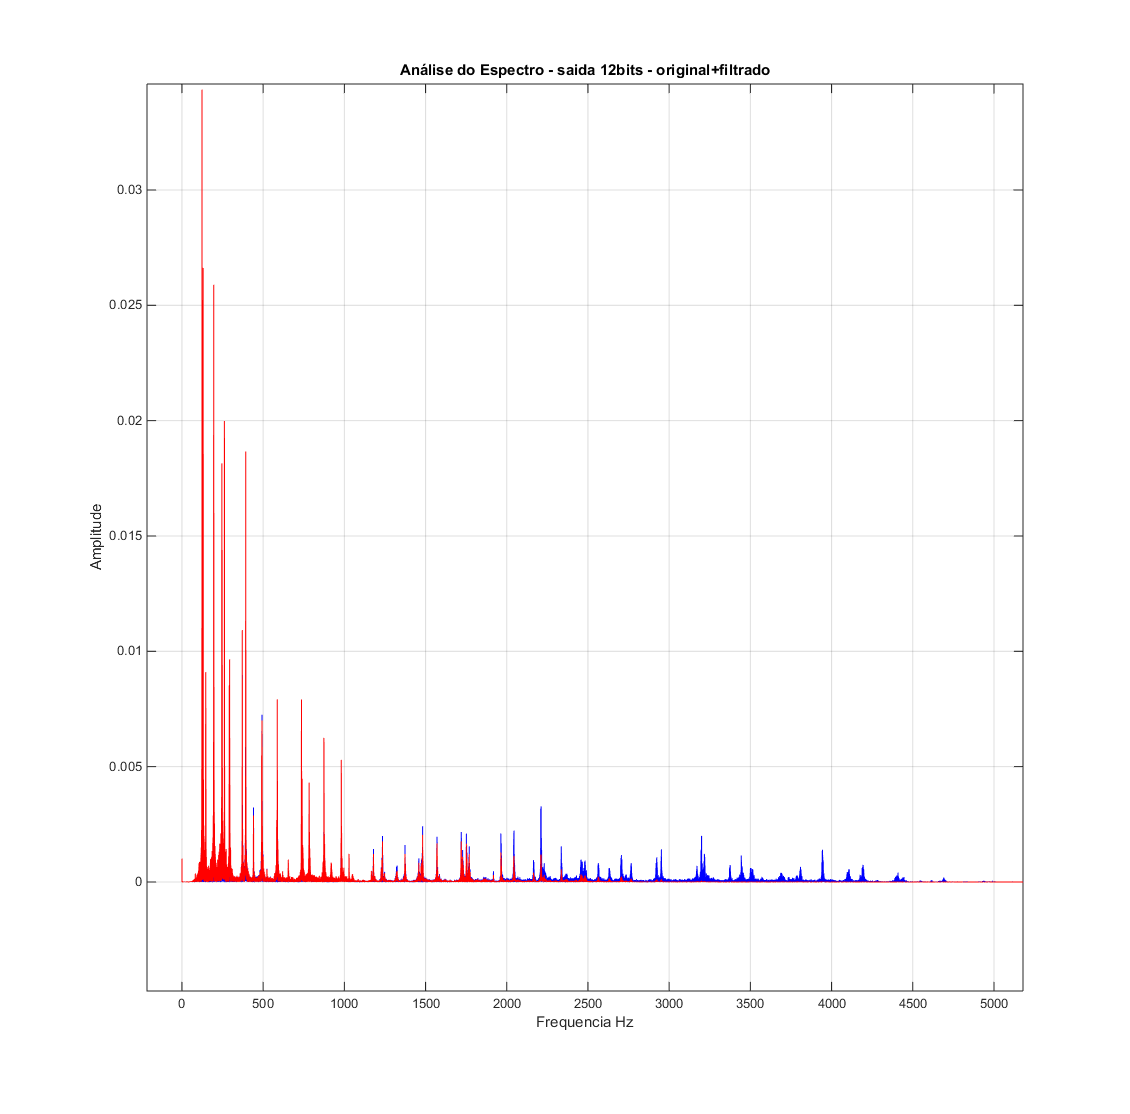
\includegraphics[scale=0.5]{./figuras/simulacoes/audio12bits-original-filtrado.png}
			\caption{Espectro de frequência do sinal original 12 bits e o sinal filtrado pelo filtro casual FIR.}
			\label{fig-sinal12bits-filtrado}
		\end{figure}
		
		
		\section{Análise dos Resultados}
			
			\subsection{Do desempenho do Código MATLAB}
			
				Avaliando a figura \ref{fig-nota-la-01} que demonstra o resultado do efeito de deslocamento seletivo em frequência (\textit{pitch-shifter}) aplicado ao sinal filtrado observamos claramente para um deslocamento de 1 oitava (para a nota A3 = 220Hz), percebemos que a resposta em frequência bate exatamente no valor que é o dobro ($ 2^{12/12} $) - A4 = 440Hz. Concluindo que o algoritmo de fato desloca em saltos de meio tom a frequência do sinal, em outras palavras, consegue alterar o \textit{pitch} do sinal sem alterar sua duração temporal.
				
				\begin{figure}[!ht]
					\centering
					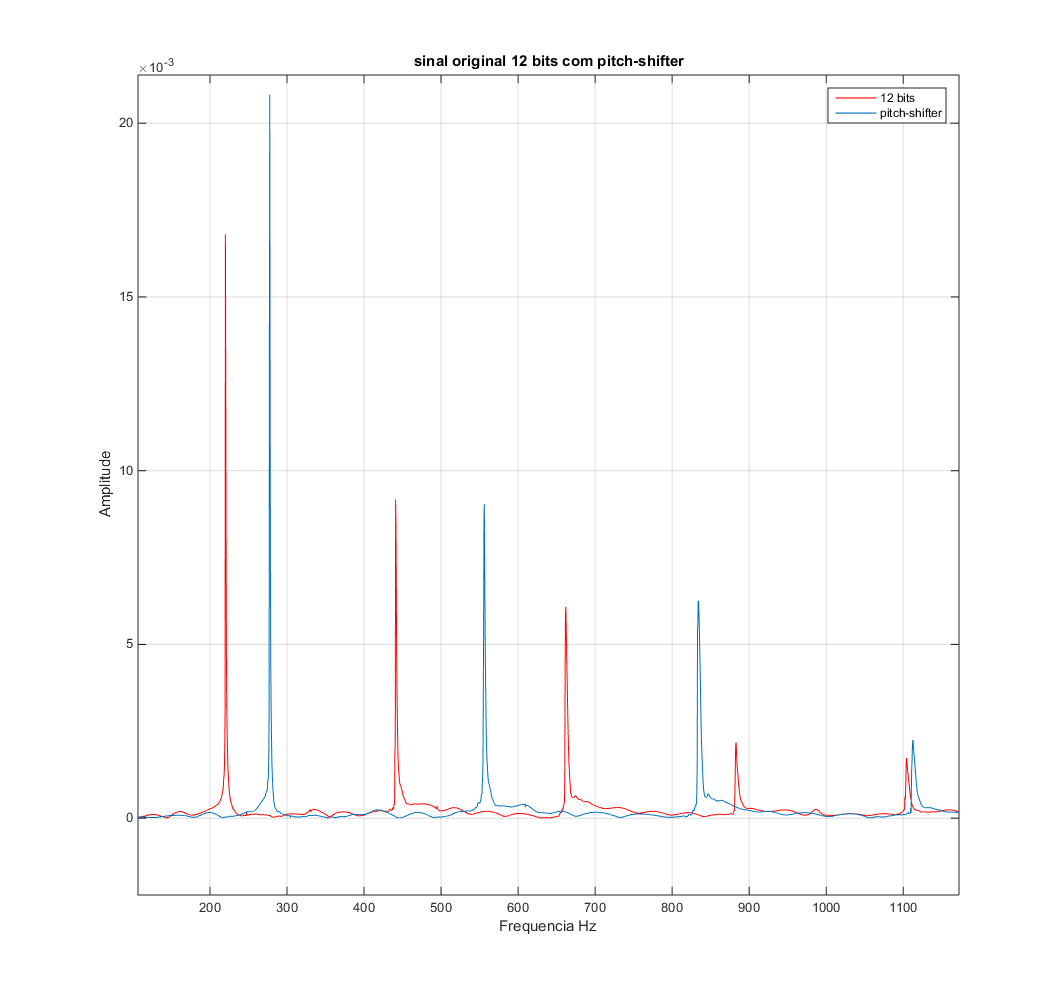
\includegraphics[scale=0.5]{./figuras/12bits-pitch-shifter.png}
					\caption{Análise espectral de um sinal puro de guitarra tocada na nota Lá - A2 = 220Hz e o efeito pitch-shifter utilizado deslocamento de 1 oitava.}
					\label{fig-nota-la-01}
				\end{figure}
				
				Não obstante, analisando o mesmo efeito só que agora com diversas notas tocadas (figura \ref{fig-nota-la-02}) ao mesmo tempo (harmonia) percebemos que o efeito tem certas diferenças em termos de amostragem das frequências que foram deslocadas do sinal. Isso é facilmente explicado e já mencionado no parágrafo \ref{parafrafo-phase-vocoder} da seção que fala sobre \textit{phase-vocoder}, que diz que a energia das frequências ora existentes entre dois segmentos de frequências (\textit{bins}) consecutivos, terá seu valor distribuído entre esses dois segmentos.
				
				\begin{figure}[!ht]
					\centering
					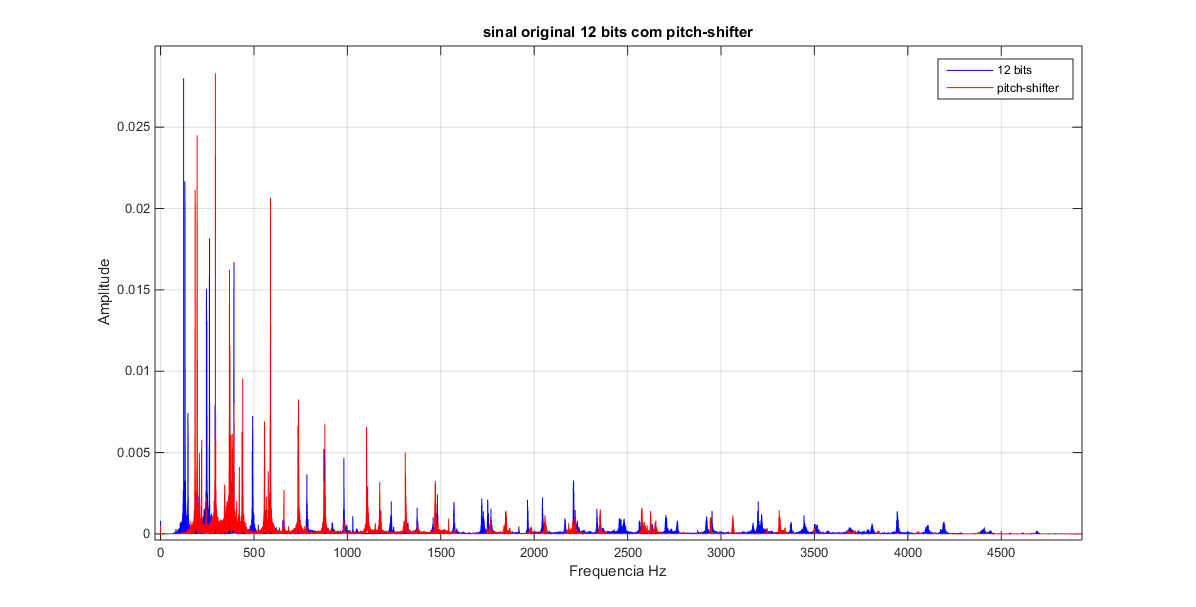
\includegraphics[scale=0.5]{./figuras/simulacoes/12bits-pitch-shift.png}
					\caption{Análise espectral de um áudio de guitarra tocando um acorde dedilhado. Pitch-shifter utilizando deslocamento de 1 oitava.}
					\label{fig-nota-la-02}
				\end{figure}
			
